\section{OD Energy Scale} \label{sec:od_energy_scale}
\par
After construction and filling of the OD, the SPE for each PMT was checked using the OD optical calibration system (OCS) \cite{lz_ocs_system_ref}.
A detailed description of the PMT monitoring during commissioning and SR1 can be found in the works of E. Fraser \cite{ewanfraser_thesis_ref}. 
During this period, an energy calibration of the OD was also performed.
Again, details of the methodology are described in \cite{ewanfraser_thesis_ref} but summarised below, as the result is used throughout this chapter to evaluate the requirements described in \autoref{sec:simulated_od_requirements}.
\par
Of the sources mentioned in \autoref{sec:lz_detector_chapter} 7 $\gamma$ sources were used.
Each were lowered into the CSD's to the 700mm level (see \autoref{fig:CSD1_Geometry}).
The sources used are summarised in \autoref{tab:od_energy_calibration_sources}.

\begin{table}[!htbp]%
    \centering
    \begin{tabular}{c|c|c}
        Source      & Specific observable         &  $\gamma$ energy (keV) \\ \hline
        ${}^{57}Co$ & direct $\gamma$             & 122                        \\
        ${}^{22}Na$ & positron annihilation       & 511               \\
        ${}^{54}Mn$ & direct $\gamma$             & 835                        \\
        ${}^{22}Na$ & direct $\gamma$             & 1275               \\
        ${}^{252}Cf$ & neutron capture on H       & 2223            \\
        ${}^{228}Th$ & ${}^{208}Tl$ $\beta-$decay & 2615            \\
        ${}^{252}Cf$ & neutron capture on Gd      & 8000            
        
    \end{tabular}
    \caption{Calibration sources used to determine the OD energy scale.}
    \label{tab:od_energy_calibration_sources}
\end{table}

\par
As discussed in \autoref{sec:od_physics}, there is a non-linear energy response in the scintillator, and therefore a non-linear energy scale below 300keV.
The empirical formula for the non-linear energy response of the scintillator from DayaBay \cite{dayabay_antineutrino_oscillation_ref, ls_nonlinear_energy_response_ref}, shown in \autoref{eq:ls_light_response}, was used to fit to these points.
\begin{equation}
    \frac{E_{vis}}{E_{true}} = \frac{p_0  + p_3 \times E_{true}}{1 + p_1 \times e^{p_2 \times E_{true}}}
    \label{eq:ls_light_response}
\end{equation}
The fit and the translation from photons detected to energy are shown in \autoref{fig:od_energy_scale}.

\begin{figure}[]
    \centering
   \begin{tikzpicture}
    \begin{groupplot}[%view={0}{90},
    group style = {group size = 1 by 2,vertical sep=0.5cm},
                   width=0.98\textwidth]
    \nextgroupplot[
            ylabel=LS energy response ($\frac{E_{vis}}{E_{true}}$),
            %xlabel=,
            xticklabels={,,}
            height=10cm, width=\textwidth,
            xmin=0, xmax=10,
            grid=major,
            ]
            %\addplot[black, smooth, domain=0:10] 
                    %{(0.00535 + 0.0286*x) / (1-0.9918*exp(-0.03018*x))};
                    %{((0.001894 + 0.03614*x) / (1-1*exp(-0.001453*x)))};
            \addplot[black, smooth]
                table[x=Energy,y=Value]
                {Data/OD_Energy_Scale/emperical_fit.dat};
                    
            \addplot[only marks,
                 error bars/.cd,
                 y dir=both, y explicit, error bar style={color=black}] table[x=Energy,y=light_response, y error=light_response_Error] {Data/OD_Energy_Scale/phd_energy.dat};

    \nextgroupplot[
            ylabel=N. photons detected,
            xlabel=Energy (MeV),
            height=6cm, width=\textwidth,
            xmin=0, xmax=10,
            ymin=0, 
            grid=major,
            ]
            \addplot[only marks,
                 error bars/.cd,
                 y dir=both, y explicit, error bar style={color=black}] table[x=Energy,y=pulseArea, y error=pulseArea_Error] {Data/OD_Energy_Scale/phd_energy.dat};
            \addplot[black, smooth, domain=0:10] 
                    {-33.98 + 0.2425*x*1000};
            
  \end{groupplot}
    \end{tikzpicture}
    \caption{OD Energy Scale and the relation between observed number of photons and the energy deposited. Analysis by E. Fraser \cite{ewanfraser_thesis_ref}.}
    \label{fig:od_energy_scale}
\end{figure}

%    \nextgroupplot[
%            ylabel=N. photons detected,
%            xlabel=Energy (MeV),
%            height=6cm, width=\textwidth,
%            xmin=0, xmax=10,
%            ymin=0, 
%            grid=major,
%            ]
%            \addplot[black]
%                    table [x=Energy,y=Value]
%                    {Data/OD_Energy_Scale/phd.dat};

\par
A comparison to other LAB-based experiments is provided in \autoref{tab:od_phe_per_mev_comparison}.

\begin{table}[!htbp]%
    \centering
    \begin{tabular}{c|c}
        Detector & phe/MeV \\ \hline
        RENO     & 150 \cite{reno_phe_per_mev_ref} \\
        Borexino & 438 \cite{pablo_mosteiro_thesis_ref} \\
        Daya Bay & 162 \cite{dayabay_phe_per_mev_ref} \\
        Kamland  & 200 \cite{kamland_phe_per_mev_ref} \\
        SNO+     & 300 \cite{snoplus_phe_per_mev_ref} \\
        LZ       & 230 
    \end{tabular}
    \caption{LZ OD photons detected per electron equivalent MeV deposited compared to other large LAB experiments.}
    \label{tab:od_phe_per_mev_comparison}
\end{table}

\subsection{Fit Uncertainty}
\par
Perhaps the largest drawback in the energy calibration is that only a single location was used, in Z.
Therefore the variation in light collection efficiency in the OD could not be taken into account, see \autoref{fig:od_lce}.
This is tested in the following Section and shown in be insignificant.


\subsection{PMT Noise}
\par
Observations of waveforms showed that there was a grounding issue, which occasionally caused high energy pulses with large PMT multiplicities.
An waveform of this is shown in \autoref{fig:noise_od_waveform} where during the noise period no physical OD event can be made out from the noise.
Included as well is an example of OD data during a quiet period of data taking showing a rate as expected.

\begin{figure}[]
\begin{subfigure}{\textwidth}
  \centering
  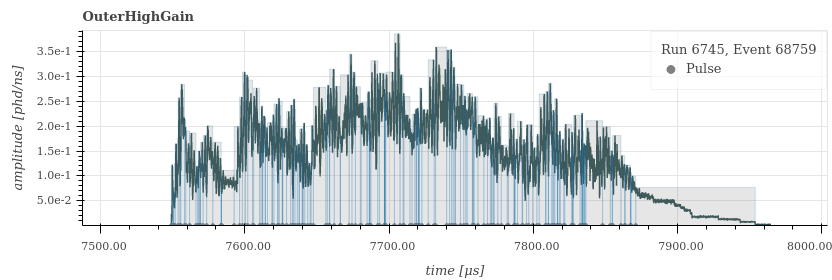
\includegraphics[width=\linewidth]{Figures/OD_Backgrounds/noise_pulse.png}
  \caption{High noise period.}
  \label{fig:noise_od_waveform}
  \end{subfigure}
  \begin{subfigure}{\textwidth}
  \centering
  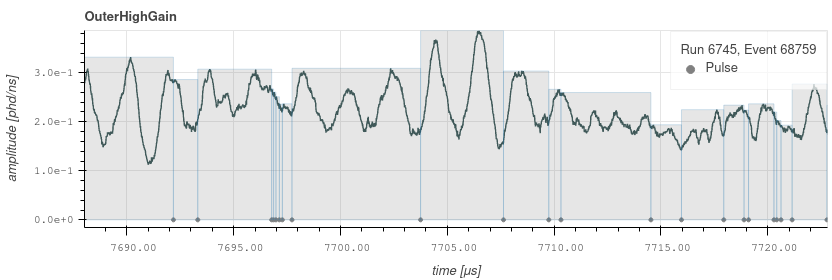
\includegraphics[width=\linewidth]{Figures/OD_Backgrounds/noise_pulse_zoomed.png}
  \caption{High noise period zoomed}
  \label{fig:noise_od_waveform_zoomed}
  \end{subfigure}
  \begin{subfigure}{\textwidth}
  \centering
  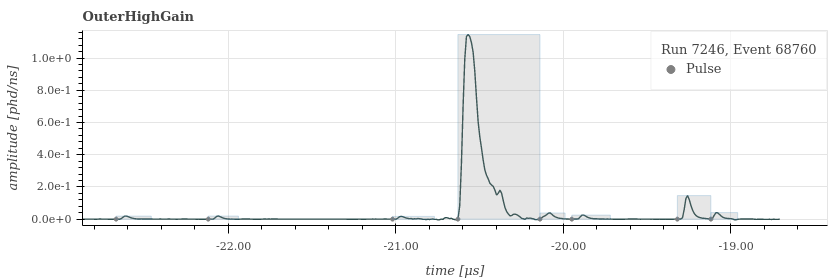
\includegraphics[width=\linewidth]{Figures/OD_Backgrounds/regular_pulse.png}
  \caption{Regular pulses}
  \label{fig:regular_od_waveform}
  \end{subfigure}
\caption{OD summed waveforms showing a noisy period of data and a regular period.}
\label{fig:od_noise_cut_waveforms}
\end{figure}


\begin{figure}[]%
\centering
\begin{tikzpicture}
\centering
  \begin{axis}[%point meta max=150,
    %point meta min=0.0,
    height=10cm, width=10cm,
    view={0}{90},
    ylabel={Pulse Amplitude/Pulse Area},
    xlabel={Pulse Area (phd)},
    xmin=0, ymin=0,
    colorbar,
    colorbar style={ylabel={Count (log$_{10}$}),},
    ]
    \addplot3[
      surf,
      shader=flat corner,
	  mesh/cols=22,
	  mesh/ordering=rowwise,
	  point meta = {z<0.1 ? nan : z}
    ] file {Data/OD_Energy_Scale/noise_cut_2d_low_2.dat};
    
    \addplot3[
      surf,
      shader=flat corner,
	  mesh/cols=30,
	  mesh/ordering=rowwise,
	  point meta = {z<0.1 ? nan : z}
    ] file {Data/OD_Energy_Scale/noise_cut_2d_high_2.dat};
\end{axis}
\end{tikzpicture}
\caption{Representative pulses seen in the OD during SR1.
         No pulse selection has been applied.
         Real events are in the distribution around 0.01 height/area.}
\label{fig:od_noise_cut}
\end{figure}

\par
In order to counteract this, a noise cut was developed to remove this based upon the pulse shape, requiring that a large portion of the pulse integral be within 100ns of the pulse starting.
Combined with a requirement of a PMT multiplicity of 5, the background noise and PMT dark rates and after pulsing were removed.
This combined selection is used throughout this chapter being referred to as the "noise cut".

\begin{figure}
    \centering
    
\includegraphics[width=0.5\textwidth]{Figures/Placeholder.png}
    \caption{Cut application}
    \label{fig:od_noise_cut}
\end{figure}

%%%%%%%%%%%%%%
\subsection{Comparison to Simulations}
\par

When data and simulations were first compared, as in Figure XXX, it became obvious that the light modelling in the OD was significantly different to reality.
Around 50\% of this difference can be accounted for by a mismatch between the PMT gains simulated against those in the LZap reconstruction database.
This effect simply results in smaller pulses and so smaller pulse areas.
However, the remaining difference is not clear where it is coming from, as it would indicate that the LCE is twice what is currently simulated (\autoref{fig:od_lce}).
In the pulse area parameter, this should remain just a linear scaling, though in other parameters (such as number of PMTs receiving light) it may not be linear.




\begin{figure}
    \centering
    
\includegraphics[width=0.5\textwidth]{Figures/Placeholder.png}
    \caption{Number of PMTs contributing to a pulse against the phe of the pulse. Or some similar plot like that}
    \label{fig:OD_coincidence_difference}
\end{figure}

\begin{figure}[]%
\centering
\begin{tikzpicture}
\centering
    \begin{groupplot}[
    group style = {group size = 1 by 2,vertical sep=2.0cm}
    ]
    \nextgroupplot[
            ylabel=Rate (Hz),
            xlabel=Pulse Area (phd),
            width=15cm,
            height=8cm,
            grid=major,
            xmin=0, xmax=700,
            ymin=1e-2, ymax=100,
            ymode=log,
            ]
        \addplot[only marks, mark size=1.0pt, error bar legend] 
            plot[error bars/.cd, x dir=both, x explicit, y dir=both, y explicit,]
            table[x=pulsearea,y=weight,x error=xerror, y error=yerror]
            {Data/OD_Backgrounds/background_constraints/od_data.dat};
        \addplot[red, const plot]
            table [x=centre,y=rate]
            {Data/OD_Backgrounds/background_fit/no_scaling/total_improved_bg_phd.dat};
        \legend{Data, Simulation};
        
            
    \nextgroupplot[
            ylabel=Rate (Hz),
            xlabel=Pulse Coincidence (PMT multiplicity),
            width=15cm,
            height=8cm,
            grid=major,
            xmin=0, xmax=120,
            %ymin=1e-2, ymax=50,
            ymode=log,
            ]
        \addplot[black, only marks, mark size=1.0pt, error bar legend,
                 error bars/.cd, error bar style={color=black},
                 y dir=both, y explicit, 
                 x dir=both, x explicit,
                 ]
            table [x=centre,y=rate,
             y error minus index=4, 
             x error minus index=6, 
            ]
            {Data/OD_Backgrounds/background_fit/no_scaling/data_bg_coincidence.dat};
        \addplot[red, const plot]
            table [x=centre,y=rate]
            {Data/OD_Backgrounds/background_fit/no_scaling/total_improved_bg_coincidence.dat};
        \legend{Data, Simulation};
    
    \end{groupplot}
\end{tikzpicture}
    \caption{Comparison of two analysis quantities; pulse area and pulse multiplicity.
             Data rates are from a single week of Random Trigger data taken during SR1.
             The simulated rates include all detector components and cavern-$\gamma$'s.}
    \label{fig:od_sim_vs_data_raw}
\end{figure}

\par
Despite this difference there are a number of ways in which data and simulations can be compared.
The simplest approach is to assume that all physics is correct in the simulation and the discrepancy can be accounted for entirely by incorrect linear scaling in the simulated PMT response.
Though this is definitely not entirely correct given the discrepancy in PMT multiplicity, and something about non-linearity in some reference...XXX...
Given the low binning in the PMT multiplicity, a simulation to data scaling has not been attempted for that here.
\par
An alternative approach to comparing simulations to data would be to translate phd into energy for both simulations and data, though generally the less manipulation that is performed on data the better.

\par
In order to calculate the scaling factor, two energies were used.
The first was from ${}^{228}Th$.
As previously mentioned, this source was used to determine the OD energy scale.
In the decay chain (\autoref{fig:decay_chains}), Tl208 has a prominent 2.6MeV $\gamma$, and features not only in the calibration run but also as part of cavern-$\gamma$'s.
Given the less clear features in the background data for cavern-$\gamma$'s of this energy, only the calibration runs were used.
Likewise simulations were performed of the decay chain in a CSD at the same position as the calibration run.
A comparison between the two pulses is shown in Figure XXX.
\par
The second scaling value was taken from ${}^{152}Gd$ $\alpha$-decays.
A much lower visible energy process that is in the non-linear region of the energy scale.
As these are an internal decay to the GdLS, variations in the light collection efficiency across the detector will be averaged out.
\par
Scaling factors were determined by fitting Gaussians to the pulse area distributions shown in \autoref{fig:od_scaling_points}.
Both methods provided similar, yet slightly different scaling values of 4.54 for ${}^{152}Gd$ and 4.77${}^{208}Tl$.
The pulse area for each pulse from simulations has been multiplied by a number of different scaling factors which can be seen in \autoref{fig:od_sim_vs_data_scaling_options}.
The result from ${}^{208}Tl$ more closely aligns simulations to data and so a value of 4.77 has been taken as the scaling factor, however, clearly there is some uncertainty on that.


\begin{figure}[]%
\centering
\begin{tikzpicture}
\centering
    \begin{groupplot}[
    group style = {group size = 1 by 2,vertical sep=2cm,
                   horizontal sep=0.4cm},
                   height=7cm, width=15cm
    ]
    \nextgroupplot[
            ylabel=Rate (Arb.),
            grid=major,
            xmin=0, xmax=50,
            ymin=1e-2, ymax=10,
            ymode=log,
            ]
            
        \addplot[black, only marks, mark size=1.0pt, error bar legend,
                 error bars/.cd, error bar style={color=black},
                 y dir=both, y explicit, 
                 x dir=both, x explicit,
                 ]
            table [x=pulsearea,y=weight,
            y error=yerror, x error=xerror]
            {Data/OD_Energy_Scale/gd152_data.dat};
        \addplot[red, const plot]
            table [x=pulsearea,y=weight,
            y error=yerror, x error=xerror]
            {Data/OD_Energy_Scale/gd152_sims.dat};            

        \legend{Data, Simulation};
            
    \nextgroupplot[
            ylabel=Rate (Arb.),
            xlabel=Pulse Area (phd),
            grid=major,
            xmin=0, xmax=800,
            ymin=1e-2, ymax=10,
            ymode=log,
            ]
        \addplot[black, only marks, mark size=1.0pt, error bar legend,
                 error bars/.cd, error bar style={color=black},
                 y dir=both, y explicit, 
                 x dir=both, x explicit,
                 ]
            table [x=pulsearea,y=weight,
            y error=yerror, x error=xerror]
            {Data/OD_Energy_Scale/tl208_data.dat};
        \addplot[red, const plot ]
            table [x=pulsearea,y=weight,
            y error=yerror, x error=xerror]
            {Data/OD_Energy_Scale/tl208_sims.dat};
        \legend{Data, Simulation};
    
    \end{groupplot}
\end{tikzpicture}
    \caption{Scaling points to compare simulations to observations in pulse area.
    The observed values are shown in black, and the simulation in red.
    \textbf{Top}: ${}^{152}$Gd from simulation and data.
    \textbf{Bottom}: ${}^{208}$Tl from simulation and data.
    Each distribution has been normalised to the bin of interest.}
    \label{fig:od_scaling_points}
\end{figure}

\begin{figure}[]%
\centering
\begin{tikzpicture}
\centering
    \begin{axis}[
            ylabel=Rate (Hz),
            xlabel=Pulse Area (phd),
            width=15cm,
            height=8cm,
            grid=major,
            xmin=20, xmax=700,
            ymin=1e-4, ymode=log,]
            
        \addplot[only marks, mark size=1.0pt, error bar legend] 
            plot[error bars/.cd, x dir=both, x explicit, y dir=both, y explicit]
            table[x=pulsearea,y=weight,x error=xerror, y error=yerror]
            {Data/OD_Backgrounds/background_constraints/od_data.dat};
            
        \addplot[red, const plot]
            table [x=centre,y=rate]
            {Data/OD_Backgrounds/background_fit/scaling_options/total_improved_scaling_4.37_phd.dat};
        \addplot[green, const plot]
            table [x=centre,y=rate]
            {Data/OD_Backgrounds/background_fit/scaling_options/total_improved_scaling_4.54_phd.dat};
        \addplot[blue, const plot]
            table [x=centre,y=rate]
            {Data/OD_Backgrounds/background_fit/scaling_options/total_improved_scaling_4.77_phd.dat};
        \addplot[purple, const plot]
            table [x=centre,y=rate]
            {Data/OD_Backgrounds/background_fit/scaling_options/total_improved_scaling_4.97_phd.dat};
            
        \legend{Data, 4.37 scaling, 4.54 scaling, 4.77 scaling, 4.97 scaling};
                
    \end{axis}
            
\end{tikzpicture}
    \caption{Comparison of observed and simulated pulse area distributions. 
             The simulated pulse areas have been scaled by a range of scaling values.
             The simulation distribution is from the expected rates described in \autoref{sec:simulated_od_backgrounds}.
             Both simulation and data are normalised to the same exposure.}
    \label{fig:od_sim_vs_data_scaling_options}
\end{figure}

